\documentclass[11pt]{article}
\title{Lenses}
\author{https://github.com/heptagons/lenses}
\date{2023/12/28}

\usepackage{graphicx}

\usepackage[margin=0.75in]{geometry}

%\usepackage{amssymb}
%\usepackage{subcaption}

\def\mathbi#1{\textbf{\em #1}}

\begin{document}

\maketitle
\begin{abstract}
Lenses are equilateral hexagons resembling optical concave and convex lenses.
\end{abstract}

\section{Lenses}

\subsection{Symmetry 5}

\begin{figure}[h]
\centering
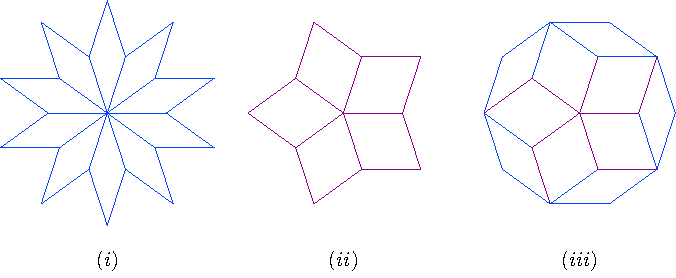
\includegraphics[scale=1.1]{bc/rhombi}
\caption{Rhombi of the types $\mathbi{b}$ and $\mathbi{c}$. The star at $(a)$ is formed with ten rhombi $\mathbi{b}$. The star at $(b)$ is formed with five rhombi $\mathbi{c}$. The regular decagon at $(c)$ is formed with five rhombi $\mathbi{b}$ and five rhombi $\mathbi{c}$.}
\label{fig:bc-rhombi}
\end{figure}

\begin{figure}[h]
\centering
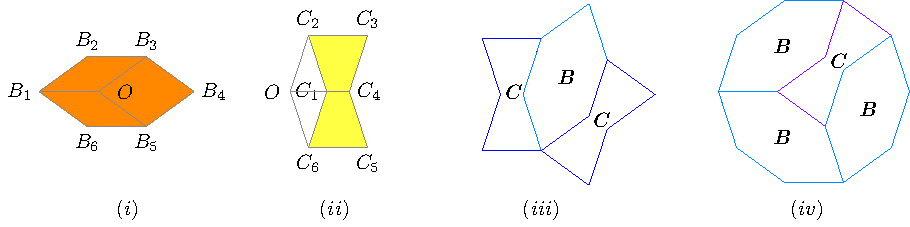
\includegraphics[scale=1.1]{bc/hexagons}
\caption{Hexagons of types $\mathbi{B}$ and $\mathbi{C}$. Hexagon $\mathbi{B}$ $(a)$ $\overline{B_1...B_6}$ area equals the area of two rhombi $\mathbi{b}$ plus one rhombus \mathbi{c}.}
\label{fig:bc-hexagons}
\end{figure}



\end{document}
